%
% Draft  document mxkde.tex
% Analysis of data from ab46 on dermal papilla cell counts
%
 
\documentclass{article}  % Latex2e
\usepackage{graphicx,lscape,subfigure}
 

\title{My experiences with MX21-KDE-x86 Linux}
\author{Neville Jackson}
\date{19 Feb 2022} 

\begin{document} 

\maketitle      

\section{Introduction} 
This investigation arose from a discussion on {\em itsFOSS} in which it became obvious that my impressions of the KDE Desktop Environment had been formed with a seriosly out of date version, way before the Plasma version. 

The decision to look at MX-KDE was based on some helpful advice, and on the need to use a very up-to-date version of KDE. MX is {\em the} most popular Linux at present, and is a member of the Debian family, with which I am familiar.

The approach taken was to pretend to be a new user of Linux, and to attempt to do everything with GUI tools. 
I also attempted to make some comparative assessments with other Linux versions and DTE's which I have installed for my normal work.

\section{Install}
\label{sec:install}
The MX21-KDE-x86.iso file was downloaded and installed to a 186Gb pre-prepared partition with an ext4 filesystem. There were existing swap spaces. The /home directory was left on the root filesystem. An existing grub2 was used to boot.

The comptuter used  was a desktop with the following hardware and software
\begin{verbatim}
System:
  Kernel: 5.10.0-9-amd64 x86_64 bits: 64 compiler: gcc v: 10.2.1 
  parameters: BOOT_IMAGE=/boot/vmlinuz-5.10.0-9-amd64 root=/dev/sda1 
  Desktop: KDE Plasma 5.20.5 wm: kwin_x11 vt: 7 dm: SDDM 
  Distro: MX-21_KDE_x64 Wildflower October 20  2021 
  base: Debian GNU/Linux 11 (bullseye) 
Machine:
  Type: Desktop Mobo: ASUSTeK model: P9X79 DELUXE v: Rev 1.xx 
  serial: <filter> UEFI: American Megatrends v: 1203 date: 05/24/2012 
CPU:
  Info: 6-Core model: Intel Core i7-3930K bits: 64 type: MT MCP 
  arch: Sandy Bridge family: 6 model-id: 2D (45) stepping: 7 
  .............
\end{verbatim}
as determined by the MXtools Quick system Info package. 
There should be no performance issues, the computer is about 10 years old but has ample cpu power and 64Gb of ram.

The approach taken was to  pretend that I was a new user wanting to do everything with GUI tools, because I wanted to see if these tools would perform for someone who had no other option.

Before proceeding I wanted to update the system.  So I hunted round for a system updat GUI and found {\em CLI APT-based Package Manager}.   It says 
\begin{verbatim}
Run apt-get update now?
\end{verbatim}
I say Yes and it just goes around a loop and asks the same question .... endlessly. Oh, I see, you have to say NO. Then it offers to do an upgrade, so I do it and it does an upgrade with output just like apt-get upgrade.  OK I got there, but it would have been quicker by hand.

{\bf Verdict:} It worked but I got confused.

{\bf Score:} About 9/10

{\bf Recommends:}  Not sure . A bit more dialog might help.

I pretended that I was a new user wanting to do everything with GUI tools, because I wanted to see if these tools would perform for someone who had no other option.

\subsection{Setup my network}
The machine has 2 ethernet ports - eth0 is a local network with printers and other computers, eth1 is connected to the ADSL modem which has DHCP. 

So {\em Settings - System Settings - Connections} and it brings up what it calls Wired Connection 1  and Wired Connection 2.  I cant tell which is which , it had set both to automatic meaning it is trying to do DHCP on both.  I have to look at {\em ip addr} and {ip route} to see what it is trying to do. I find it has a working connection to the modem on Wired Connection2, and the other is non functional.

I try to set Wired Connection 1 to static with an IP address and netmask using the GUI menu. It fails.  I cannot ping anything on the local network.

I think the GUI is using NetworkManager. Trying to manage both networks with NetworkManager ( ie with the GUI) is a bad idea. So I decide to only let NetworkManager manage the DHCP link, and to make the local network static and controlled by thef-up/if-down system.

So, I have to setup the /etc/networkj/interfaces file as follows
\begin{verbatim}
# The loopback network interface
auto lo
iface lo inet loopback

# The primary network interface
# eth1 is under NetworkManager

# The local private network
auto eth0
iface eth0 inet static
    address 192.168.32.6
    netmask 255.255.255.0
\end{verbatim} 
Then I boot the machine, and let NetworkManager bring up only one connection, this time it calls it Wired Connection 1, and it works. And now the local static network works too. 
There is no sign of a Wifi connection.  I do have a WiFi port, but the GUI cant find it . The {\em ip} command can find wlan0, so if I wanted that I would probably have to set it up outside the GUI too. 
 
I tried the obvious experiment, disconnect the ethernet connection to modem and see if the GUI finds the WiFi connection - it doesnt find it. 

Then I discover the bottom panel has a  button called {\em Networks} and it sees both the wired connection eth1 and  the WiFi connection to the modem, and I can enable the WiFi connection from there. If I enable both the WiFi and eth1 I get 2 default routes, which is OK.

Then with both eth1 and WiFi connections turned on in the panel, I go back into the KDE GUI, and now it lists both Wired connection1 and the WiFi connection to modem. Wow. How was I supposed to know to setup the panel first and then use the KDE GUI?

{\bf Verdict:}  Hardly a triumph for the Connections GUI, but I think the problem is it depends on NetworkManager which is notoriously difficult, and it does not seem to deal with WiFi connections unless they are turned on first in the lower panel. Having Networks in the panel as well as a Connections GUI is confusing.

{\bf Score:} about 3/10

{\bf Recommends:} The following changes to GUI are needed
\begin{itemize}
\item   It needs to label the connections with something intelligable like {\em Intel 82579V Ethernet or eth1}
\item It needs to deal with WiFi without depending on the Panel - it has {\em Connections} ( which seems to mean all connections) and {\em Bluetooth}  but no {\em WiFi}  appears in the listed connections until WiFi is turned on in the panel.
\item It should offer the user some choice before diving into NetworkManager. If it had a preliminary screen which simply listed all the connection hardware and asked the user for some tips about what they wanted for each interface, then it might be able to setup NetworManager sensibly. Alternatively, and less desirably, it might {\em direct} the user to the existence of the panel.
\item The MX Network Assistant goes some way towards this. It lists all the interfaces , properly labelled, but it does not offer to accept any user input and it does not link up to  the KDE Connections menu.
\end{itemize}
Networking seems to always be made more difficult than it should be. There is base information ( like what are the interfaces and what do you want to do with them) and there are prrocedures ( ways of configuring). Network GUI's seem to always mix these 2 things up and thereby confuse the user. All the user should need to be involves in is is the base info. The rest should be able to be logically automated.

\subsection{Setting up OKI Postscript printer}
This is a very simple printer to setup because it has inbuilt postscript and there are drivers present in just about every Linux version. So lets see if we can do it with the GUI.

So {\em Settings - System Settings - Printers} then
Add new printer, and it discovers OKIPage12i and MFC640CW. Choose OKIPage12i, and it brings up 192.168.32.99 and Port 9100. The IP address is right, it is an ethernet printer. Never seen Port 9100 before, so ignore it. Choose a driver Okipage12i Foomatic/Postscript from the list, name it OKI, and set a s default printer. All looks correct so print a test page , and it prints an error sheet!!

Go thru it all again, cant see anything else to set , so go back to CUPS localhost:631 page. Set it all up again with CUPS, then right at the end I notice Papersize is set to {\em letter}. Change to {\em A4}. Print test page, and it works.

So why didnt the GUI offer me a menu item to set the Papersize? That is fairly basic.  Go back and check - it really is not there in the GUI.

{\bf Verdict:} The GUI fails to configure the printer

{\bf Score:} About 1/10. 

{\bf Recommends:} It would be an easy fix. Just add a menu item for Papersize, or at least a warning message.  There is another way - in Void Linux clicking on the {\em System settings - Printers} menu just brings up the CUPS localhost:631 page which is a bit less friendly than the KDE GUI, but it least it has all the neessary functions.

\subsection{Setting up Brother multifunction printer}
This is also an ethernet connected printer, but it is not Postscript, it requires drivers. The drivers are not available in any Linux distro I know of, one has to download them from the Brother site. 

I have done this  lots of times. I have to check for presence of some directories, install the csh shell, then use dpkg to install the drivers which are .deb files., and finally copy some libraries into /usr/lib32. There is no GUI for any of that so I just do it.

Then do as for OKI printer in {\em Settings - System settingd Printers}. It does all that OK, finds the drivers I installed. At end I print a test page , and this time I get a test page to print but half ogff the edge of the page. Clearly the papersize is wrong again. So back to CUPS, fix the papersize, and it prints test page correctly. 

{\bf Verdict:} The GUI fails for same reason as for OKI printer.

{\bf Score:} About 2/10

{\bf Recommends:} Add a papersize setting to GUI menu.


\subsection{Mounting filesystems}
I need to mount another filesystem on /dev/sda4,  automatically, every time it boots. The GUI that does mounts seems to be Dolphin. Dolphin can find the partition and will mount the filesystem for the current run, but it does not seem to have any menu choice to do an automount.  There is also the MX-Tools Disk Manager GUI, it is the same - ie it will do an in-session mount, but not an automount.

I am not surprised that a GUI is not provided for this. Editing {\em /etc/fstab}  is one of the easiest ways to lock yourself out. One slip and it will not boot. 

So, I very carefully make a mount point called {\em /common}, make a backup copy of fstab, edit it adding one line to mount {\em /dev/sda4} to {\em /common} . Reboot, and it works. 

{\bf Verdict:} I had to use the command line here, but there is a good reason.

\subsection{Adding a directory to the search path}
I want to add {\em /home/nevj/bin} to my PATH. There seems to be a tool for this. So I open {\em System - Bash Config} select {\em Executable paths} and add {\em /home/nevj/bin}, exit and do {\em echo \$PATH} , and it is not there. 
Then I remember, you have to either use {\em source .profile} or reboot to get {\em bash} to read its {\em .profile}. So reboot, and {\em echo \$PATH} again, and it is there now. 

{\bf Verdict:} Well at last something works

{\bf Score:} About 9/10

{\bf Recommends:} It would have been nice to warn the first time user that they had to reboot for it to take effect.

\section{Usage using GUI tools}
\label{sec:usage}

\subsection{File Manager}
I want to look at that fstab file I edited, so lets try out {\em Dolphin}. I move it to {\em /etc} then double click on {\em fstab} and great, it displays the contents of {\em fstab} in a {\em KWrite} window. I then try the same with {\em fstab.orig} and it says it cant determine the file type and brings up a popup of things I might want to open the file with. That is nonsense, it is a text file, almost identical to {\em fstab}.  Go away and think. Try again next day , and it is OK - ie Dolphin displays both files correctly. How can it change?

Much fiddling around, I decide to do a simple test. Make a file called {\em txt.txt} with a few lines of ASCII text. Copy it to three other files {\em txt.jpg} {\em txt.pdf} and {\em txt.orig}. Check their file types
\begin{verbatim}
nevj@trinity:~
$ file txt*
txt.jpg:  ASCII text
txt.orig: ASCII text
txt.pdf:  ASCII text
txt.txt:  ASCII text
nevj@trinity:~
$ 
\end{verbatim}
Start Dolphin. {\em txt.txt} and {\em txt.orig} display correctly in a KWrite window, but {\em txt.jpg} attempts to display in a {\em Gwenview} window and gets the message {\em Loading txt.jpg failed} and {\em txt.pdf} attempts to display in an {\em okular} window which can display text so it works. Boot and try again, still the same.

So  I determine that {\em Dolphin} seems sometimes to be using the 'extension' part of the filename to determine its type. Why ?  That is Microsoft nonsense. Unix filesystem does not work like that, Unix uses the {\em file} command to determine file types, and extensions can be anything or not even present. I also dont understand this intermittant behaviour?  Is the system taking time to sort out file types in background?

I accept that it is nice for a graphical File Manager to identify file types, so it can display them with a click.  But for goodness sake, why cant Dolphin use the {\em file} command instead of extensions. 


{\bf Verdict:} Has to be a fail. We want it to correctly identify Unix file types.

{\bf Score:} About 4/10, it looks OK otherwise.

{\bf Recommends:} Use {\em file} command to determine file types in Dolphin. Find why this issue is intermittant?

\subsection{\LaTeX install}
I want to install \LaTeX \hspace{1pt} to write this document. So lets give the MX Package Installer a try. Start MX Package Installer, choose Stable Repo, search for texlive,
install texlive, and a heap of additional packages.  Installs all work first go.

I am going to need a pdf viewer, so also install evince. Then discover okular is nearly the same, so lets use okular.

This doc was written in  \LaTeX \hspace{1pt} using {\em vi} in the konsole terminal window, Pdf output was from {\em pdflatex} from the texlive package. I used {\em okular} to dynamically view pdf output. Everything worked

{\bf Verdict:} All OK

{\bf Score:} 10/10

{\bf Recommends:} The MX package Installer is a bit plain as GUI, but it functions.

\subsection{R install}
This time I decided to try Discover, which is a KDE package management GUI.  Discover is a much more upmarket GUI than MX Package Installer. You can search for applications in categories, and it segregates application addons, and plasma addons (what are they?). 

So search for {\em r-cran} and it finds R and R-commander. Install R and everything goes smoothly. What you get is an R icon under Science and Math and also under Graphics. Start up R using the icon -- and it brings up R in a Konsole window.  Where is it in the filesystem?
\begin{verbatim}
> system("pwd")
/home/nevj
> 
\end{verbatim} 
It is in my home directory.  That is crazy! It suggests a complete lack of understanding of the way R is used and how workspaces are accessed and saved.

The basic approach of all R users is that you {\em cd} in a terminal window to the directory for the project you want to work on, then open R there , so that it accesses and saves its workspace (which is a file called .RData) in that directory. This keeps workspaces for various projects separate, and, more importantly, stops you from running 2 copies of R with the same workspace. 

So what the icon does  is useless to any R user who wants to work on more than one project, and is actually {\em dangerous} because it is possible to hit the icon  twice and start two copies of R running, both in the home directory which would result in workspace corruption.

What did it install?
\begin{verbatim}
> sessionInfo()
R version 4.0.4 (2021-02-15)
Platform: x86_64-pc-linux-gnu (64-bit)
Running under: Debian GNU/Linux 11 (bullseye)

Matrix products: default
BLAS:   /usr/lib/x86_64-linux-gnu/blas/libblas.so.3.9.0
LAPACK: /usr/lib/x86_64-linux-gnu/lapack/liblapack.so.3.9.0
\end{verbatim}

OK, so it used R-4.0.4 ( same as Debian 11) but it used the R BLAS libraries. I wanted the OpenBLAS libraries - ie like I get in Debian shown below
\begin{verbatim}
> sessionInfo()
R version 4.0.4 (2021-02-15)
Platform: x86_64-pc-linux-gnu (64-bit)
Running under: Debian GNU/Linux 11 (bullseye)

Matrix products: default
BLAS:   /usr/lib/x86_64-linux-gnu/openblas-pthread/libblas.so.3
LAPACK: /usr/lib/x86_64-linux-gnu/openblas-pthread/libopenblasp-r0.3.13.so
\end{verbatim}

That is a mystery. How can MX be in line with Debian 11 for R , but not use the update-alternatives facility to offer alternative BLAS libraries. 

Might sound trivial, but it is important to anyone who does liear algebra in R

 
{\bf Verdict:} Very poor effort. Not KDE specific, all DTE's treat R like this. We can do better.

{\bf Score:} About 1/10 for GUI  and that is generous.

{\bf Recommends:} The icon should bring up a preliminary window in which the user can set the working directory, define the things that normally go in the .First file and .Last file, give access to the {\em R CMD ...}  statement and well as plain {\em R} with options,  and perhaps set packages to be loaded. There is an opportunity for KDE to do much better here.


\subsection{Julia install}
Julia has a different workflow ethic to R. The Julia REPL (read, evaluate, print loop) is just that; it does not have a workspace which it saves automatically to a file, like R. With Julia you keep the *.jl files and other data in a directory and manage them with your favourite editors, Unix file utilities, etc. You can either {\em include} .jl files into the REPL to execute them, or run them as scripts. 

So Julia is not as fussy about where it runs as R. Lets see how an install goes. We use {\em MX Package Installer} this time. Go to Stable Repo, search for julia, a bit slow but it finds it, do install - it scrolls output across the screen , just like apt-get, finishes successfully .  A Julia icon appears in Science and Math. 
 
Start Julia with the icon - it brings up a Konsole window, just like R, and again in the home directory.

{\bf Verdict:} Same issue as R but not as serious.  It still lets me start two Julias in the same directory.  It offers no choice of working directory. 

{\bf Score:} About 5/10. OK but could do a lot better

{\bf Recommends:}  Make a startup window that offers user a few choices, like which directory to work in, set julia command options,  execute a source file. I know there are environments like {\em jupyter} but that is no excuse for installing an icon that does nothing.

\subsection{Vi usage}
I often use {\em view} which is part of {\em vi} to look at large text files, because it is safe - it opens the file in read only mode.. It also scrolls around better than {\em more}. So {\em view mxkde.tex} and up comes another window ( unexpected) with a weird top and bottom panel? 

After some trial and error I determine that it is loading the {\em Midnight Commander editor} which happens to also be called {\em view}. So there is a name clash.

After using {\em vi} awhile, I discover that if I am insert mode and the mouse focus leaves the window to do something else, and then I return to vi, it is no longer in Insert mode? I dont want that behaviour. 
{\bf Verdict:} Easily fixed. Remove {\em Midnight Commander editor}. Then my {\em vi} version of {\em view} works. Would a novice have worked this out?

{\bf Score:} About 5/10. 

{\bf Recommends:} MX ought to be more careful about clashes.

\section{Comparative assessments}
We now want to look at things other than "does it work?". Things like "does it promote a good workflow" , " is it easy on the eyes", "is there any artistic quality". These can only be done comparatively. So I have to line it up against some of my other installations and make some subjective judgements.

I have
\begin{itemize}
\item MX/KDE
\item Debian/Gnome
\item Devuan/Xfce
\item Solus/Budgie
\item Void/Xfce
\end{itemize}
Set up some scores
\begin{description}
\item[workflow] anyone can make a clutter by invoking too many objects and arranging them poorly. We have to take that factor out of it  and try and assess how well each DTE helps me to be tidy and makes it easy to access tools. 
\item[look] things important for "easy on the eyes" are night redshift and color balance and not having to move things frequently.
\item[feel] artistic quality almost impossible to describe. It means "do I feel happy using it" or "is it interesting" or simply "do I react positively"
\end{description}
 I attempted to rate each of my installations for the above attributes on a score of 1 to 10, 10 being best. My scores, which are highly subjective, are shown in Table~\ref{tab:scores}
% latex table generated in R 3.4.2 by xtable 1.8-2 package
% Tue Jan 30 21:03:37 2018
\begin{table}[ht]
\centering
\caption{Subjective scores for Workflow, Look, and Feel of five desktop environments}
\label{tab:scores}
\begin{tabular}{|rrrr|}
 \hline
 \vspace{2pt}
 & Workflow & Look & Feel \\ 
  \hline
  \vspace{2pt}
MX/KDE & 6 & 8 & 7 \\
Debian/Gnome & 7  & 8 & 6 \\
Devuan/Xfce & 8 & 4 & 5 \\
Solus/Budgie & 7 & 8 & 9 \\
Void/Xfce & 8 & 4 & 4 \\
   \hline
\end{tabular}
\end{table}



Basically the minimal desktops (Xfce) encourage tidiness and easy workflow, the ones with redshift (KDE, Solus, and Gnome) are superior for night work, and the one that excites me most is Solus, although KDE is a good second. There must be some artistic talent on the Solus team, the Solus Software Centre is outstanding - way ahead of all contenders. Xfce needs to catch up on redshift, it will never feel wonderful, but it wins in making things simple. One thing that helps with workflow is being able to restore the previous session on reboot. Only Xfce and KDE can do this, as far as I can determine.

We will finish with some screenshots. Figure~\ref{fig:mxkde} shows the MX-KDE default screen with the {\em Discover} package utility GUI displayed.
%\documentclass{article}
%\usepackage{graphicx,subfigure}
%\begin{document}

\begin{figure}[!h]
  \centering
   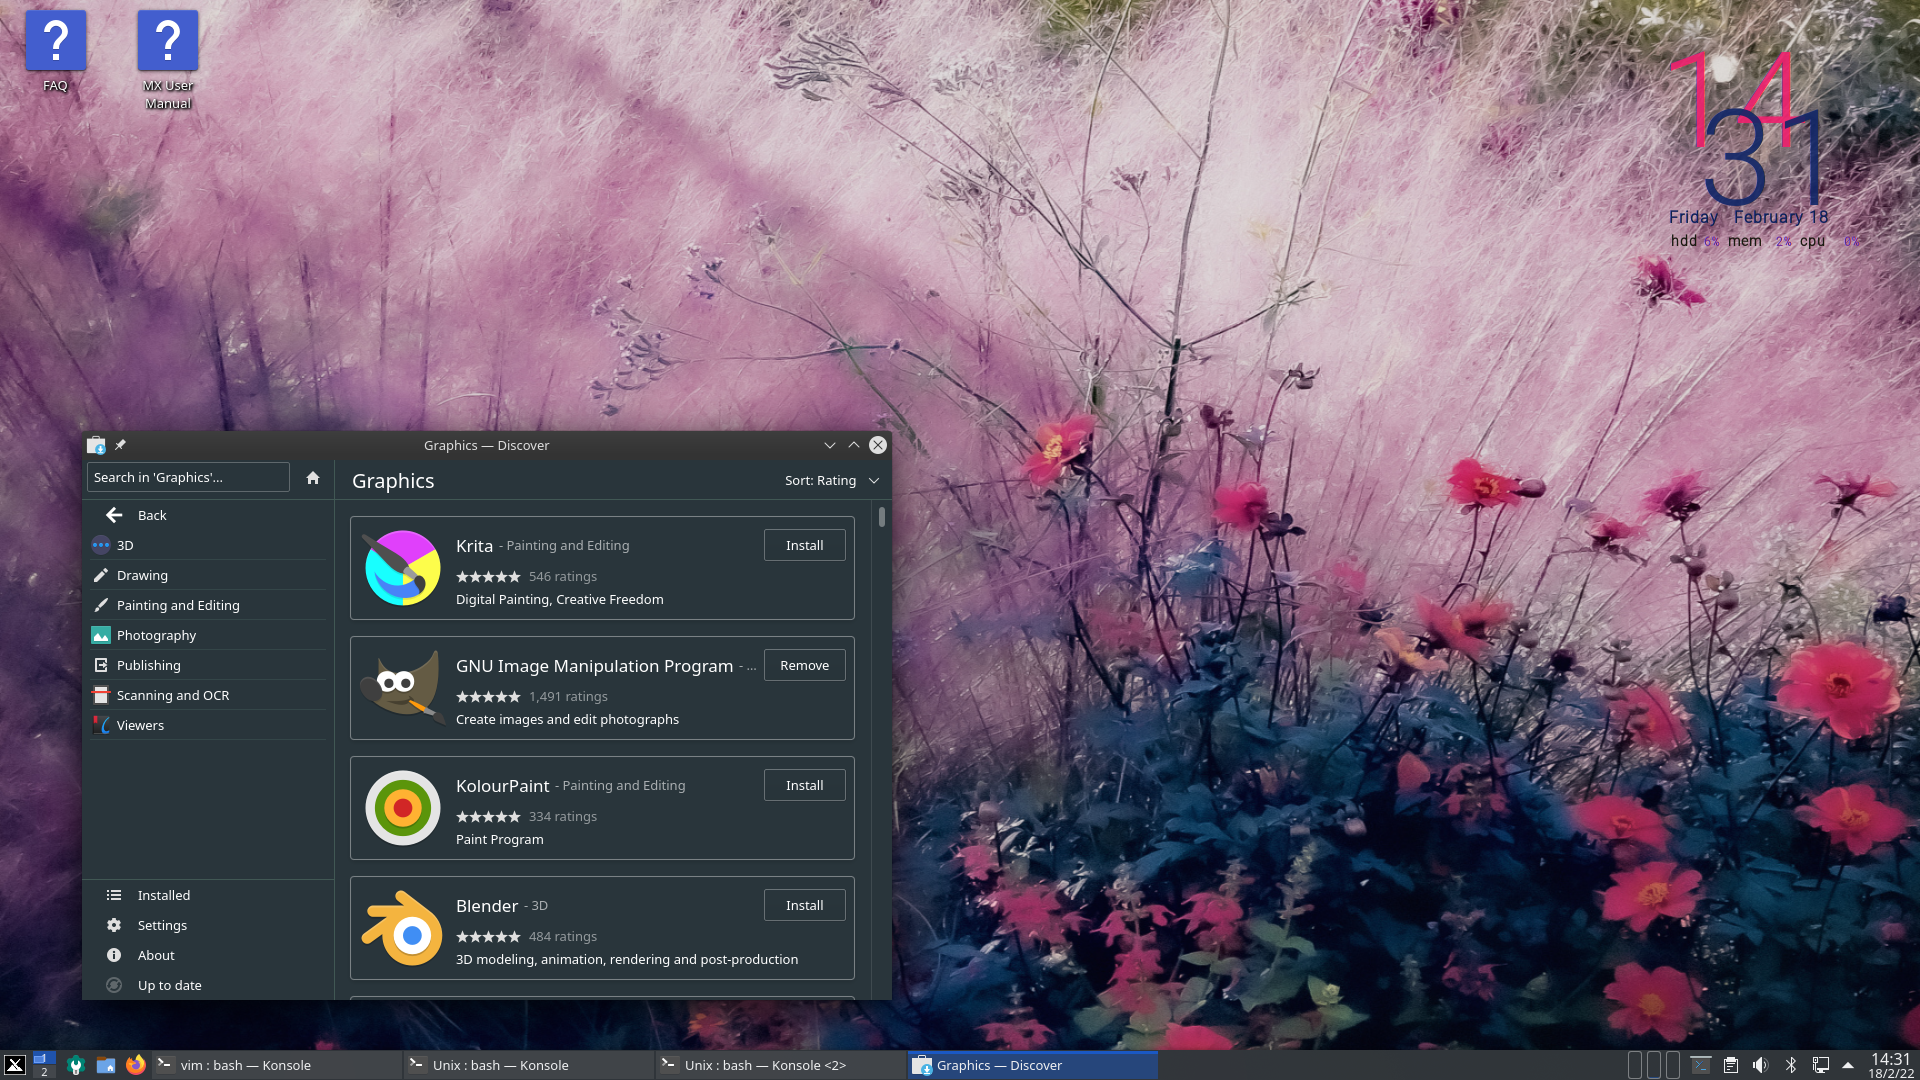
\includegraphics[width=0.9\textwidth]{mxkdescreen.png}
  \caption{Screenshot of MX21-KDE showing the {\em Discover} package window on a default background}
  \label{fig:mxkde}
\end{figure}

%\end{document}


{\em Discover} is quite well put together, and easy to use.  There is also the MX Package Installer, which is very plain.

I am trying to get the next image, so I mount the Solus filesystem with {\em Disk Manager} . That mounts to {\em /media/sda7}. Then I want to view the available shots, so I use {\em Gwenview} , and it cannot access the mnounted filesystem - /mnt does not appear anywhere in its {\em Places} menu?

So - very poor integration between Gwenview and  Disk Manager. Hang it I will just copy them all across to my workspace here and sort it out locally.  Solved it after many trials. You have to open Gwenview with the command line in the mounted directory, then it can see the files within the mount - rather messy!

Figure~\ref{fig:solusbudgie} shows the default Solus/Budgie screen with the Solus Software Management System GUI displayed.
%\documentclass{article}
%\usepackage{graphicx,subfigure}
%\begin{document}

\begin{figure}[!h]
  \centering
   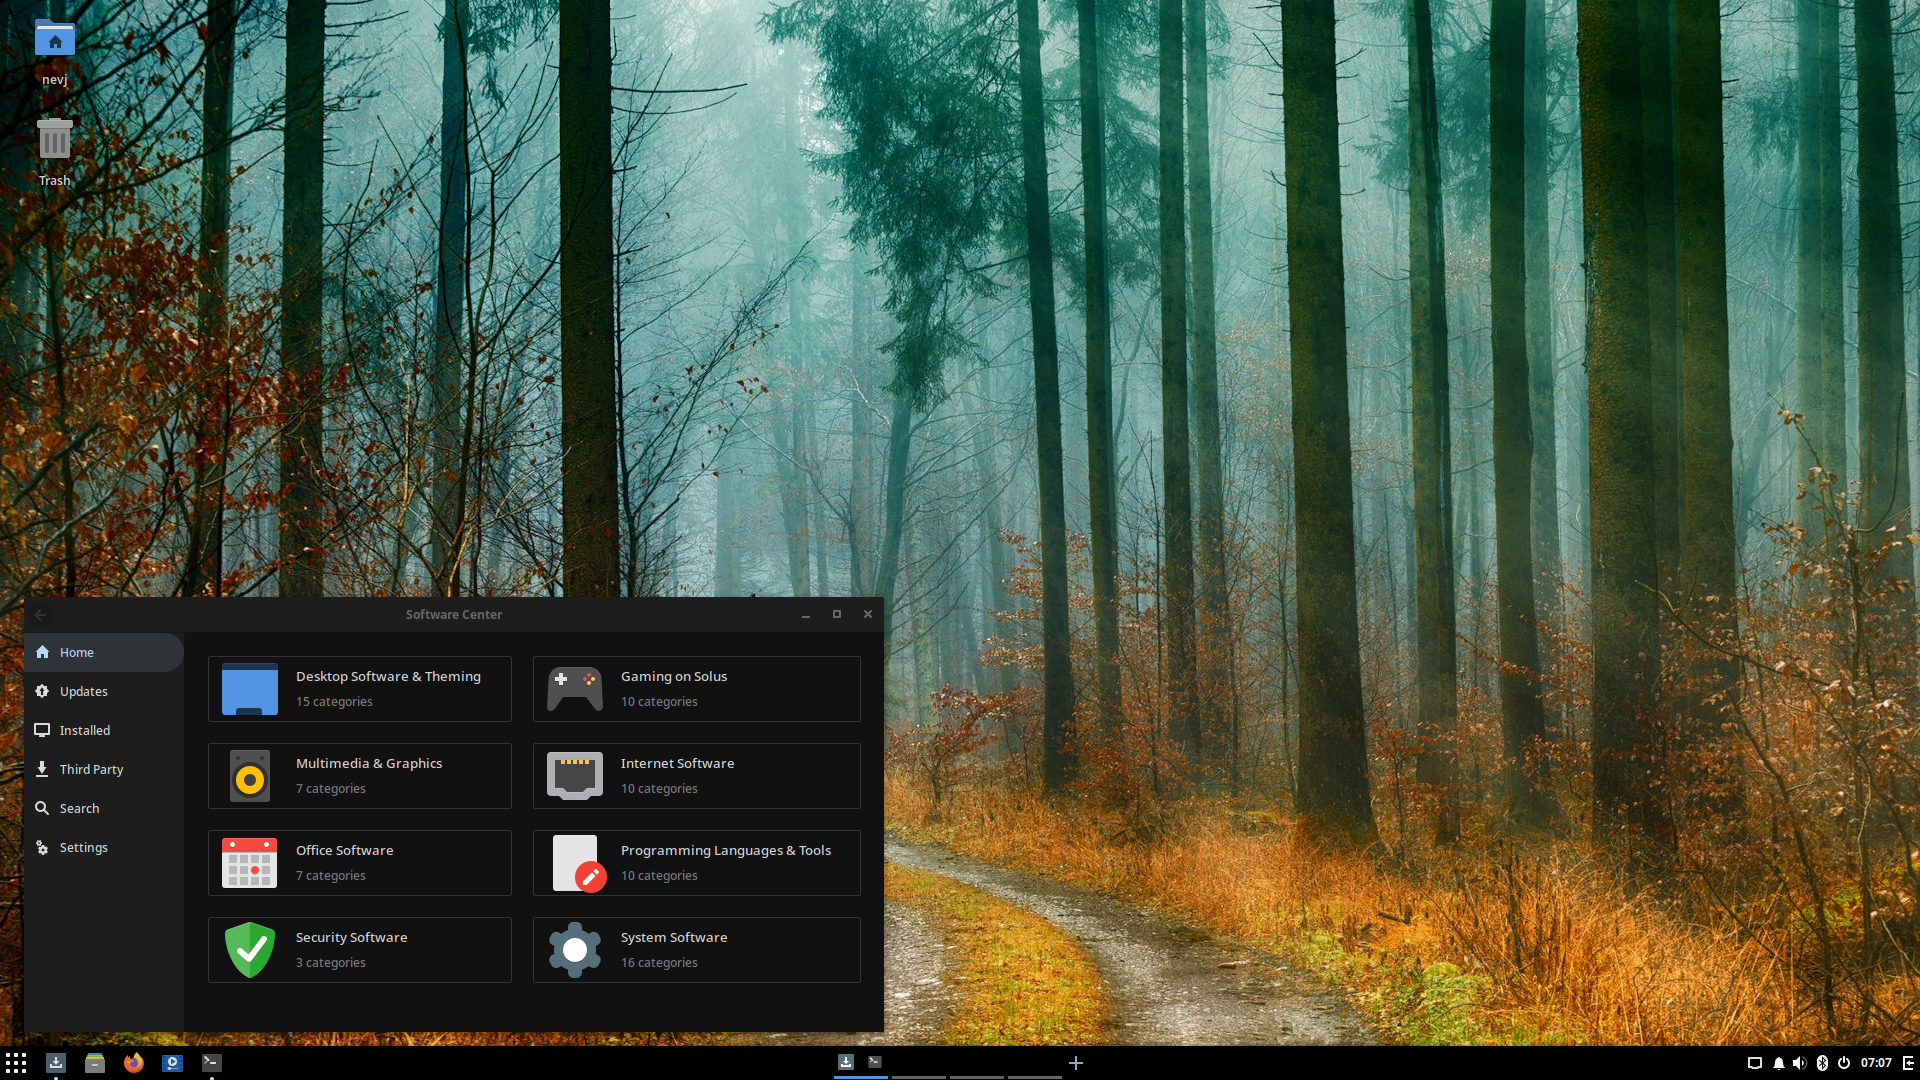
\includegraphics[width=0.9\textwidth]{solusbudgiescreen.png}
  \caption{Screenshot of Solus/Budgie  showing the {\em Solus Software Centre} package window on a default background}
  \label{fig:solusbudgie}
\end{figure}

%\end{document}


The Solus Software Management System GUI is very impressive, best I have seen. When you search out a package it brings up a description and for many packages a screenshot - right there in the package manager.

Figure~\ref{fig:voidxfce} shows the default Void/Xfce screen with a termninal window and the Void artwork added.
%\documentclass{article}
%\usepackage{graphicx,subfigure}
%\begin{document}

\begin{figure}[!h]
  \centering
   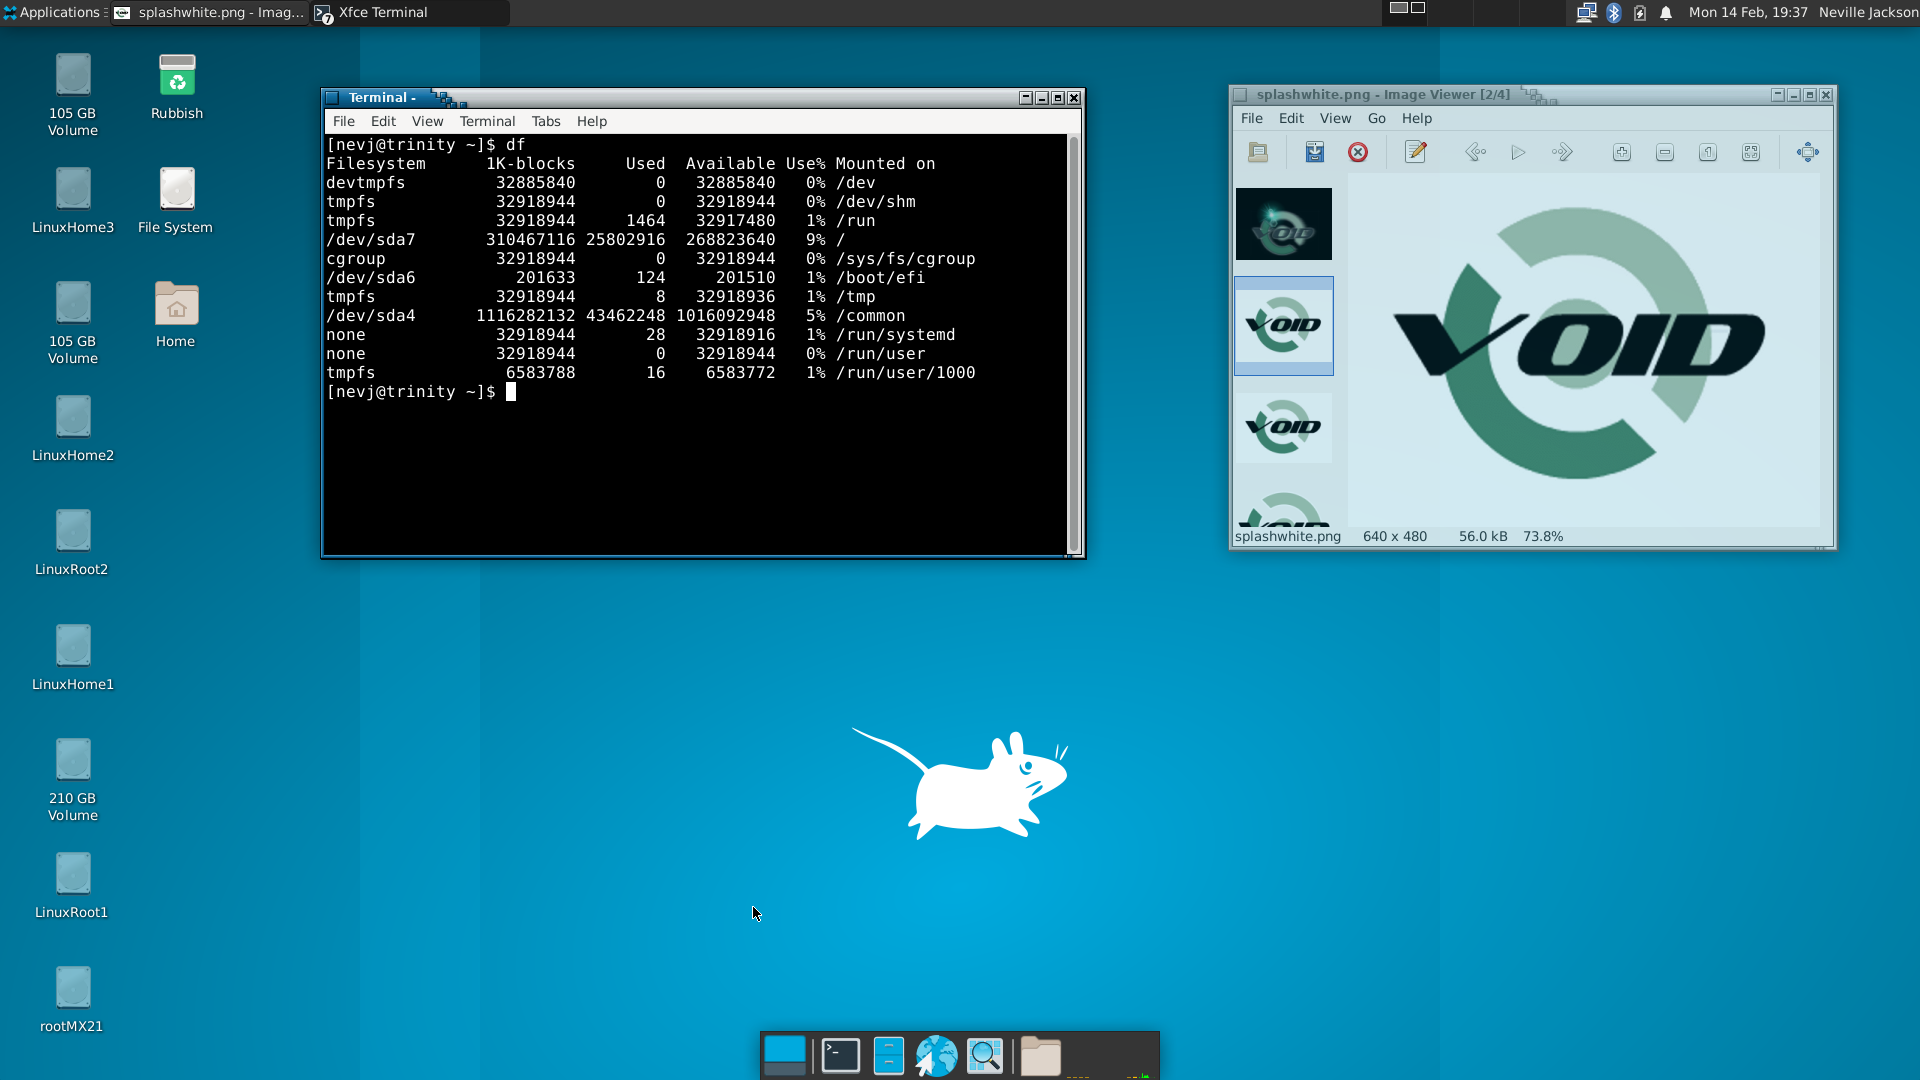
\includegraphics[width=0.9\textwidth]{voidxfcescreen.png}
  \caption{Screenshot of Void/Xfce  showing a termial window and the Void artwork on a default background. There is no package manager GIU in Void, it is command line only}
  \label{fig:voidxfce}
\end{figure}

%\end{document}


 Void has no GUI for package management, you have to use the {\em xbps} commands in a terminal. The commands are simple and the package system works well, but there is no GUI.

Figure~\ref{fig:debiangnome} shows the default Debian 11 Gnome 3 screen with the Synaptic Package Manager added.
%\documentclass{article}
%\usepackage{graphicx,subfigure}
%\begin{document}

\begin{figure}[!h]
  \centering
   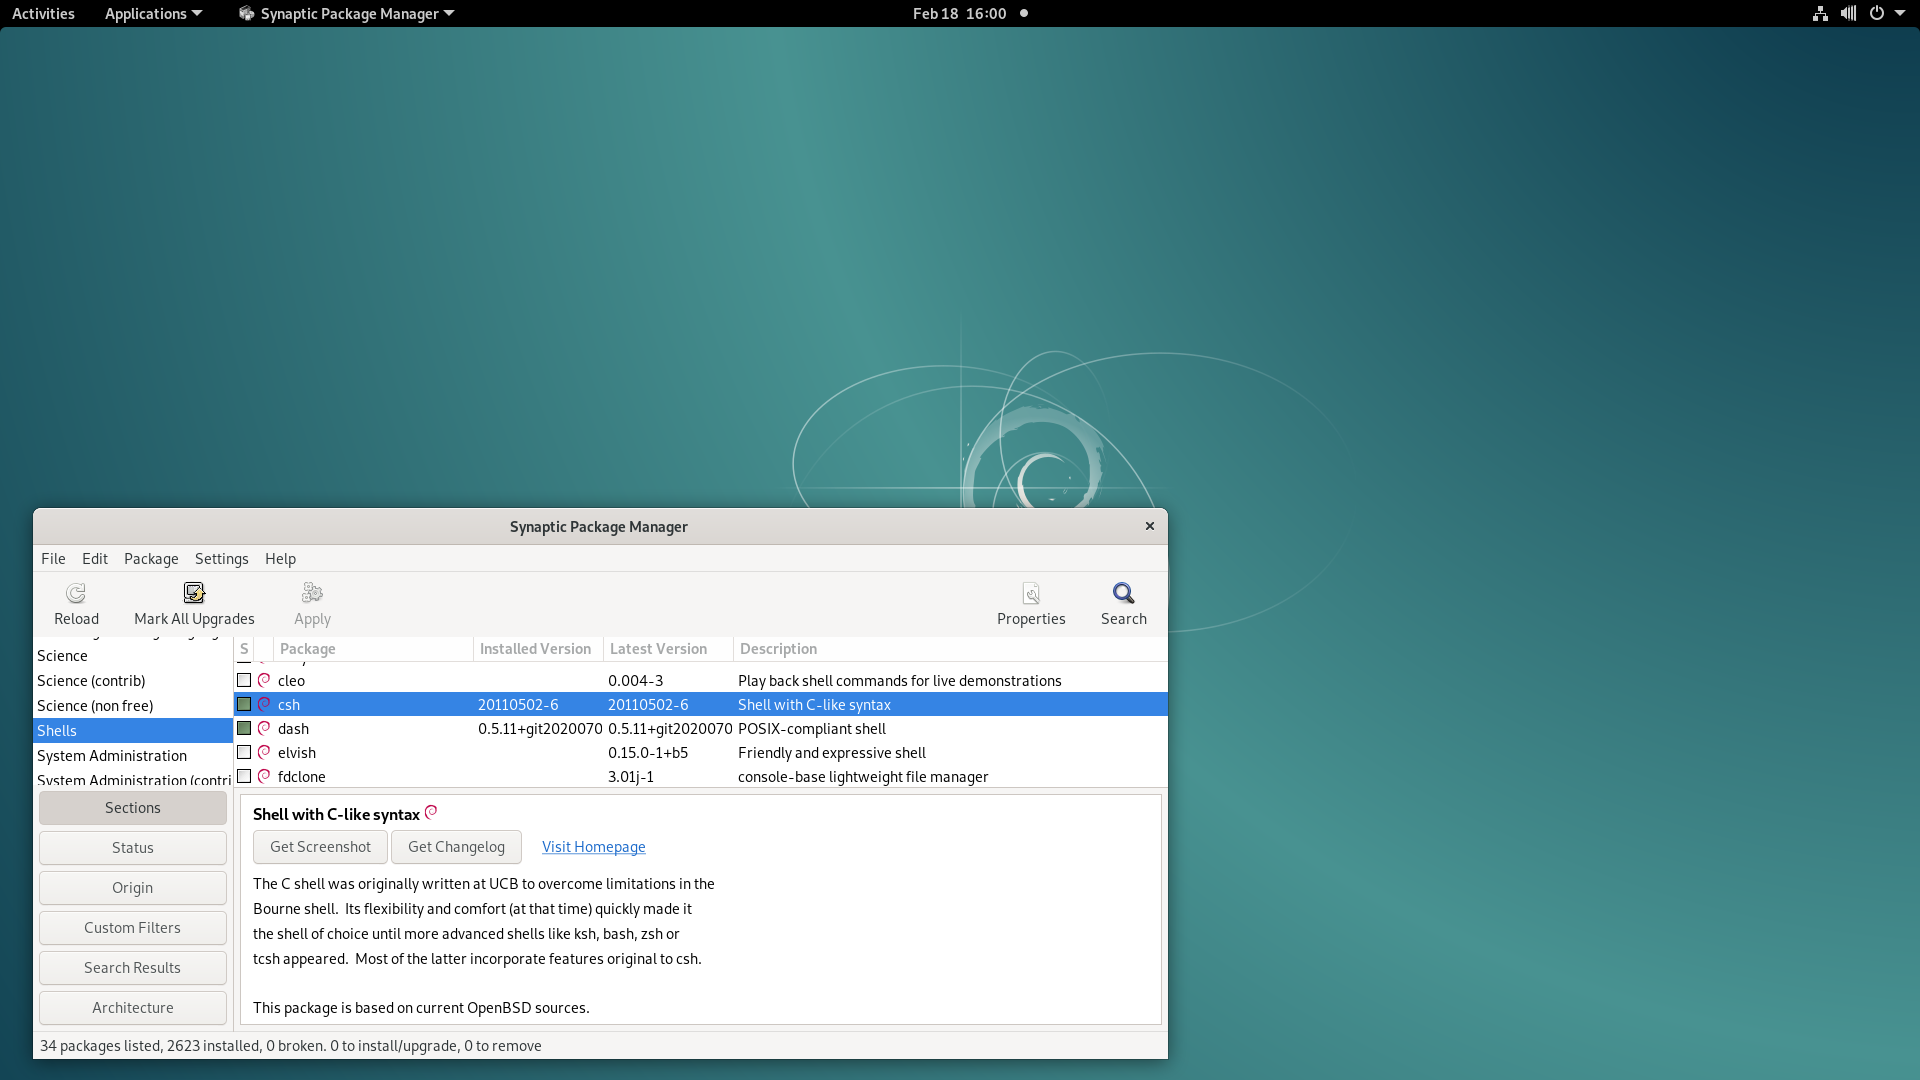
\includegraphics[width=0.9\textwidth]{debiangnome.png}
  \caption{Screenshot of Debian 11 with Gnome DTE  showing the Synaptic Package Manager and the default Debian background}
  \label{fig:debiangnome}
\end{figure}

%\end{document}


Synaptic is quite plain compared to Solus/Budgie or Mx/KDE pagkage managers. but it is longstanding and functional. I think most Debian users shun it and use the {]em apt} commands.

Figure~\ref{fig:devuanxfce} shows the Devuan 4 Xfce 4  screen with Synaptic Package Manager added. 
%\documentclass{article}
%\usepackage{graphicx,subfigure}
%\begin{document}

\begin{figure}[!h]
  \centering
   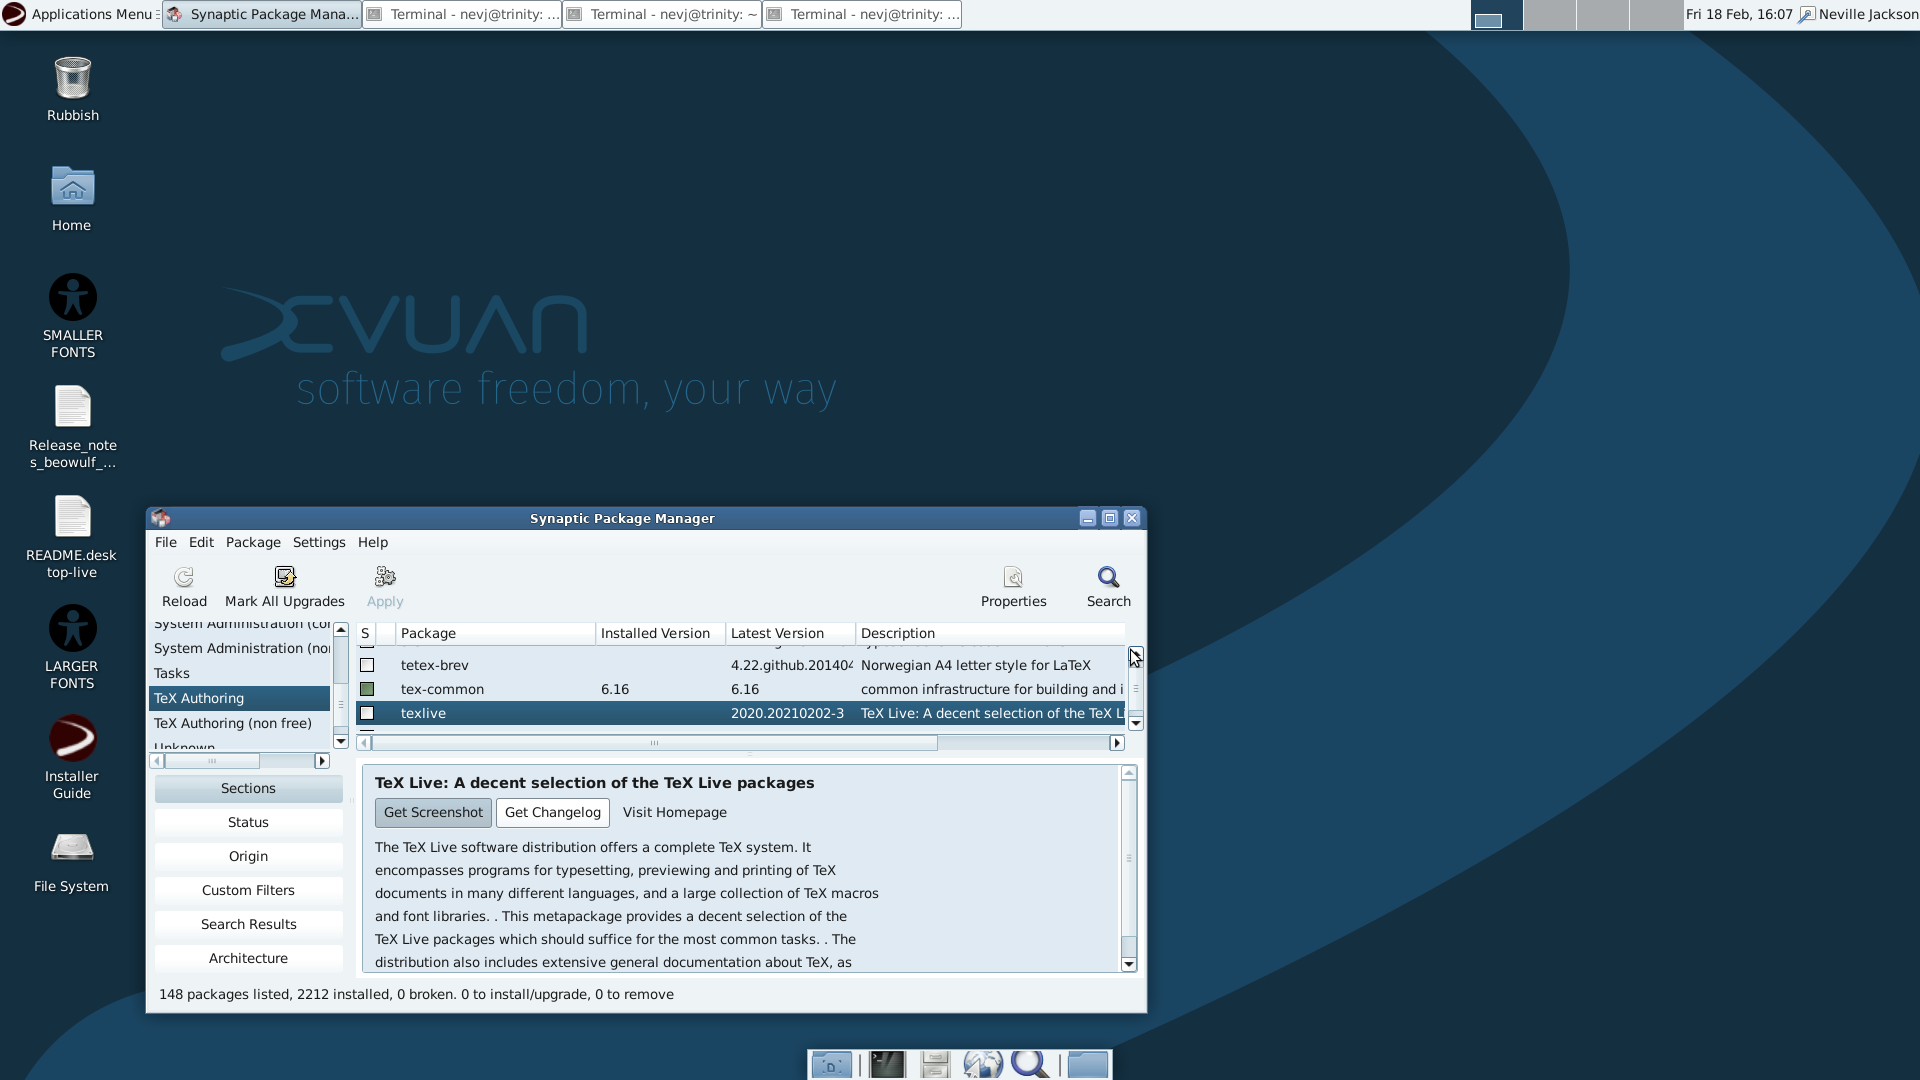
\includegraphics[width=0.9\textwidth]{devuanxfce.png}
  \caption{Screenshot of Devuan 4 with Xfce DTE  showing the Synaptic Package Manager and the default Devuan background}
  \label{fig:devuanxfce}
\end{figure}

%\end{document}


Devuan is similar to Debian, but the presentation is a bit more enhanced. It is hard to know whether this is Xfce against Gnome, or Devuan against Debian. They are both rather plain compared to Solus/Budgie or MX/KDE.

I hope the screenshots show something of the look and feel of the various DTE's and how I came to score them as in Table!\ref{tab:scores}. It is not feasable to show everything and I am unable to illustrate workflow.


\clearpage
\section{What are these plasmoids and how can I use them?}
Well, after 3 weeks using KDE I have yet to discover a plasmoid. For something that is supposed to be a lead feature of KDE/Plasma desktop, it is rather invisible.  I will have to give in and read the manual.

OK, read up a bit,  the desktop and panel are basic containments that can contain widgets.  That is just renaming things, other DTE's do the same.. I wanted to know about those extra plasmoid things.  I will say one thing, MX comes with reasonable documentation., but KDE Help Center is a bit sparse, and the terminology keeps shifting - are they plasmoids, or applets, or widgets?.

I found the {\em Add Widgets} item on the background menu, and managed to add  {\em Bluetooth} widget to the main background area of the screen. It minimised all my windows, but that is recoverable. So now I have a bluetooth background widget which does exactly the same as the bluetooth panel widget. In other words I didnt need it, so rub it out after finding out I had to use {\em Enter Edit Mode}.  The learning curve is a bit steep.

 Had a browse thru all the widgets. They all seem to be like mini-windows with no controls, but they will do I/O. I might be able to use that.  None of the widgets offered seem essential to me, but I can see that I could use the concept to control and maybe to receive R graphics output. But how do I set up a widget? Well based on my X11 days, it is some sort of programming job, but where are the tools? 

Well, I found the Plasma Addon Installer. There is {\em Command output} , {\em Configurable button},  {\em Scriptinator},  ...  maybe I could use one of those, or maybe I need to program?

Hang on, what is this Conky thing? It seems to have something to do with managing widgets. The {\em About} popup is not helpful, it says "Utility for managing Conky configuration files". I am none the wiser.  I can see {\em conky} is running.  Search of KDE Help Centre says conky has a Unix man page. 
\begin{verbatim}
conky(1) - A system monitor for X originally based on the torsmo ...
\end{verbatim}
Read man page for conky(1). It seems to be about drawing things on the screen from C - like the X11 libraries?  No it is more about system stuff?  I have to resort to Wikipedia to find out what it really is. Not directly relevant.

I tried {\em Command Output}. Installed from the Download New Plasma Widgets window. It appears now in Add Widgets menu. Select and install. And yes, I can write a command output on a panel.

That is enough. I will give Plasma Addons a pass.  THis is not the place for a full investigation. They are obviously useful for monitoring things that are changing with time.

On the general idea of having plasmoids on the screen as well as in the panel, I can only acknowledge that it is new and unique to KDE. It is not all that radical a change but it is something, and it may be able to be tailored into something very special in particular cases.

\section{Discussion}
My overall reaction to KDE today? Well it is very difficult for a large development like KDE to escape from its past, and KDE has almost the longest history of all DTE's. I can remember in the 1990's deciding it was too big for my modest 486 running FreeBSD. It is much bigger now, but computers now have ample capacity and I have no problem with its size or speed in my setup.  Some of its features, however, reflect its original design - prefix everything with 'K' or rename it completely, put in multiple tools for the same job,  and end up with large pulldown menus of applications. Other things are new or changing - panel design, plamsmoid widgets, and the quqlit of applications has improved enormously. That 'pin' on the windows reminds me of Openlook and workspaces are, of course a modern development made possible by improvements in memory and graphics interfaces. The actual window manager is invisible, buried behind the DTE somewhere - it was once the only thing present. Modern DTE's do much more than manage windows.

The KDE team have done really well to get it up to or slightly better than the other modern DTE's. Other newly written DTE's like Solus/Budgie have not been constrained by history and it shows in them being able to develop a unique and artistic style of presentation. That would always be much more difficult for KDE, but I would rate it a good second to Solus/Budgie in these matters.

The important thing about KDE is that it is going somewhere. As long as its development is active it should remain one of the DTE's of choice for Linux users.  There will always be niche requirements , like ultra-lite DTE's, which it cannot fill without extensive pruning, but for normal and high end users wanting a GUI with lots of options, it fits well. 

The issues raised in Sections~\ref{sec:install} and ~\ref{sec:usage} would be likely to have trapped a novice user.  I was able to get around all except the issue with {\em vi} insert mode and mouse focus interacting. Most of the GUI issues could be improved with a bit of work and design care. There is room for improvement yet in KDE and in all DTE's.
 
\end{document}
